\documentclass[tikz]{standalone}
\usepackage[utf8]{inputenc}
\usepackage{amsmath}
\newcommand{\altura}{.45cm}
\usetikzlibrary{calc}
\usetikzlibrary{backgrounds}
\def\hash{\mathrm{H}}

\begin{document}

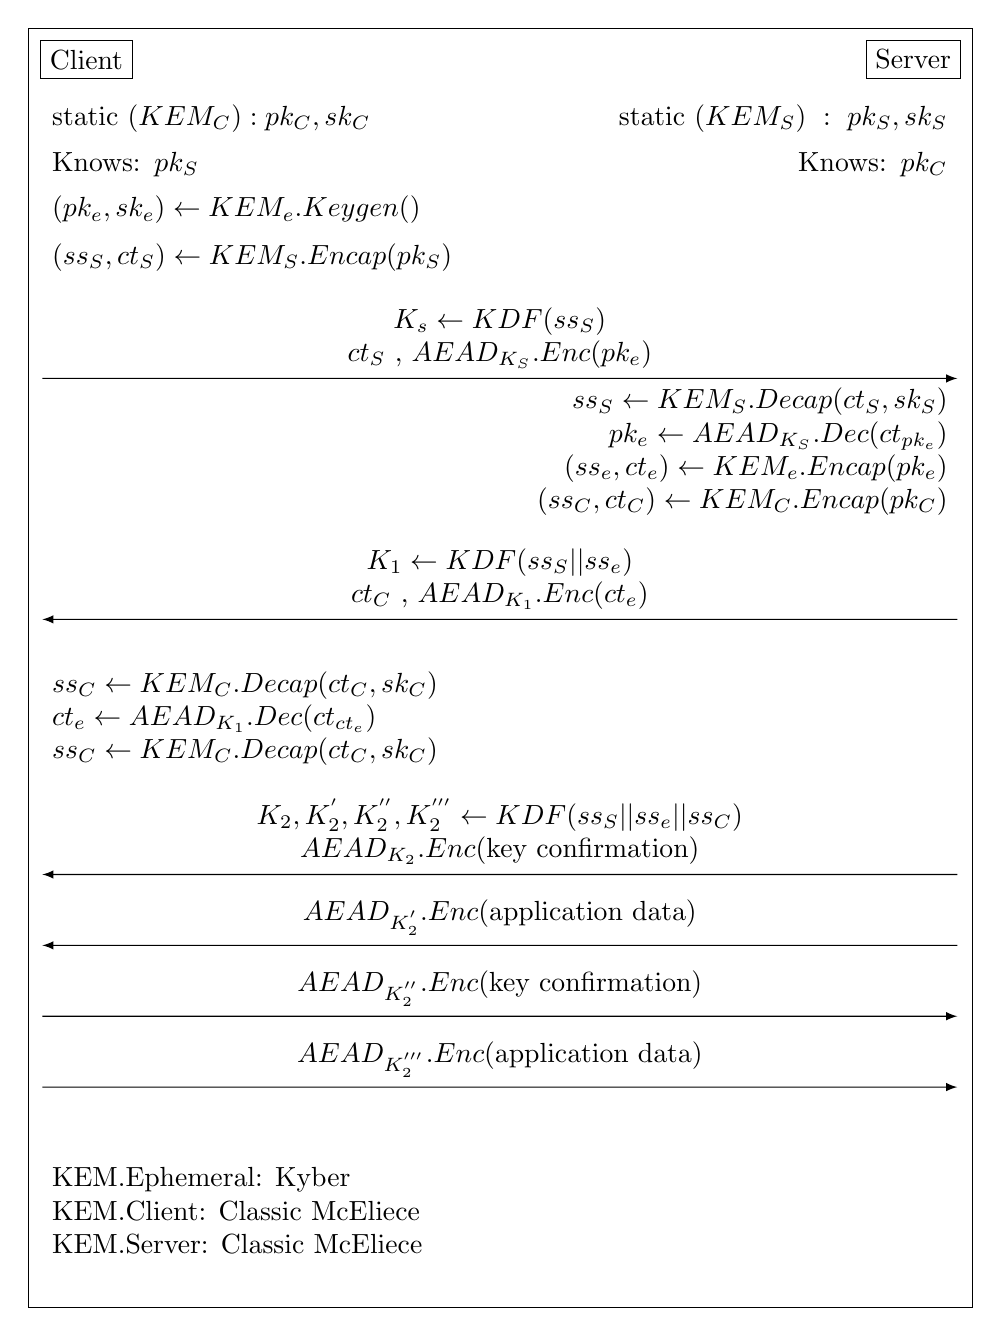
\begin{tikzpicture}[yscale=.9,xscale=.7,framed]
\tikzstyle{box}=[draw,fill=white, rectangle, rounded corners=3pt, align=left, minimum width=5.7cm, minimum height=.8cm]
 \tikzstyle{nome}=[draw, rectangle,anchor=west, minimum height=\altura,minimum width=9cm]
% Public parameters and password
%\node[draw=none,fill=none,align=center] (public) at (0,1.2) {%
%\vbox{\halign{\hfill# & # \hfill\cr
%Public parameters:& prime number $p$,base $g$, parameter $k$\cr
%Password:& $x = \hash(\text{salt}, \text{id}, \text{pw})$\cr
%}}};
  
% Client: generate public data
%\draw (-10,0) node (Client) {Client };
\node (client) at (-10,0)  [draw] {Client}; 
\coordinate (C) at (-10.8,-0.5);
\coordinate (S) at (5.8,-0.5);
%\draw[thick] (Client) -- ++(-5, -15);
\node (StaticC) [below right,align=left,text width = 10cm] at (C.south){static ($KEM_C): pk_C,sk_C$};
%\usepackage{fixltx2e} 
%like\textsubscript{this}
%were made by \emph{accident}.
\node(kA)[below,text width = 10cm] at (StaticC.south) { Knows: $pk_S$};
\node (initCkg) [below,text width = 10cm] at (kA.south) {($pk_e,sk_e) \gets KEM_e.Keygen()$};
\node (initCencap) [below,text width = 10cm] at (initCkg.south) {($ss_S,ct_S) \gets KEM_S.Encap(pk_S)$};
\coordinate (InitEnd) at (-10.8,-4.5);
\coordinate (InitSEnd) at ($(S.south) + (0, -4)$);
%$ x_{12345} \quad x_12
% Server: generate public data
\node (server) at (5,0) [draw]{Server};

\node(StaticS) [below left,align=left,text width = 5cm,align=right] at (S.south) {static ($KEM_S): pk_S,sk_S$};
\node[below,text width = 5cm,align=right](kB) at (StaticS.south) { Knows: $pk_C$};
%\node[below right , align=left] at (Server.south) {secret: $v:= g^x$ \\ other: salt};

\draw[-latex,align=center] ($(InitEnd.south) $) -- (InitSEnd) node [pos=0.5, above](handshake1) {$K_s \gets KDF(ss_S)$\\$ct_S$ , $AEAD_{K_S}.Enc(pk_e)$};
\coordinate (hs1End) at ($(InitEnd.south)+(0,-3.4)$);
\coordinate (hs1SEnd) at ($(InitSEnd.south) + (0, -3.4)$);
% Client and Server: generate secret key
\node[below left, align=right] (processServer) at (InitSEnd.south) {$ss_S \gets KEM_S.Decap(ct_S,sk_S)$\\  $pk_e\gets AEAD_{K_S}.Dec(ct_{pk_e})$\\ ($ss_e,ct_e) \gets KEM_e.Encap(pk_e)$ \\$(ss_C,ct_C)\gets  KEM_C.Encap(pk_C)$};

\draw[-latex,align=center] (hs1SEnd.south)  -- (hs1End.south) node [pos=0.5, above](handshake2) {$K_1\gets KDF(ss_S||ss_e)$\\$ ct_C$ , $ AEAD_{K_1}.Enc(ct_e)$};
\coordinate (hs2End) at ($(InitEnd.south)+(0,-4)$);
\coordinate (hs2SEnd) at ($(InitSEnd.south) + (0, -4)$);

\node[below right, align=left] (processClient) at (hs2End){$ss_C \gets KEM_C.Decap(ct_C,sk_C)$\\$ct_e\gets AEAD_{K_1}.Dec(ct_{ct_e})$\\$ss_C\gets KEM_C.Decap(ct_C,sk_C)$};

\draw[-latex,align=center] ($(hs2SEnd.south) + (0, -3)$) -- ($(hs2End.south) + (0, -3)$) node [pos=0.5, above]{$K_2,K_2^{'},K_2^{''},K_2^{'''}\gets KDF(ss_S||ss_e||ss_C)$\\$AEAD_{K_2}.Enc$(key confirmation)};
\draw[-latex,align=center] ($(hs2SEnd.south) + (0, -4)$) -- ($(hs2End.south) + (0, -4)$) node [pos=0.5, above]{$AEAD_{K_2^{'}}.Enc$(application data)};
\draw[-latex,align=center] ($(hs2End.south) + (0, -5)$) --  ($(hs2SEnd.south) + (0, -5)$)node [pos=0.5, above]{$AEAD_{K_2^{''}}.Enc$(key confirmation)};
\draw[-latex,align=center]  ($(hs2End.south) + (0, -6)$) -- ($(hs2SEnd.south) + (0, -6)$) node [pos=0.5, above]{$AEAD_{K_2^{'''}}.Enc$(application data)};
\node[below right, align=left] (captions) at ($(hs2End.south) + (0, -7)$){KEM.Ephemeral: Kyber\\KEM.Client: Classic McEliece\\KEM.Server: Classic McEliece\\};
 
% verification if the session key is the same
%\node[box,below] (verifServer) at ($(processClient.south) + (10,-1)$) {Verify $M_1$\\ $M_2 \gets \hash(A, M_1, s_k)$};
%\node[box,below] (verifClient) at ($(verifServer.south) + (-10,-1)$) {Verify $M_2$};

% labels on arrows

%\draw[-latex,thick] ($(kB.south) + (0, -1)$) -- ($(initClientkg.south) + (0, -1.5)$) node [pos=0.5, above] {$B$, salt};

%\draw[-latex,thick] ($(processClient.south) + (0, -.5)$) --++ (10, 0) node [pos=0.5, above] {$M_1$};
%\draw[-latex,thick] ($(verifServer.south) + (0, -.5)$) --++ (-10,0) node [pos=0.5, above] {$M_2$};

\end{tikzpicture}

\end{document}